\chapter{Lane Following}
In this chapter we present a Lane Following alghorithm based on Adaptive Model Predictive Control. First we introduced the case-study model, then we designed the controller and the overall procedure scheme. Finally we verified the proposed strategy in different scenarios considering a double lane change, sinusoidal and elliptic/circular paths.
\section{Problem Formulation}
A lane-following system is a control system that keeps the vehicle traveling along the centerline of a highway lane, while maintaining a user-set velocity. Figure \ref{fig:laneFollowing} illustrates a typical lane following scenario.
\begin{figure}[!h]
	\centering
	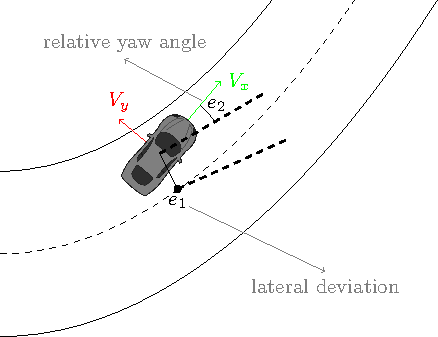
\includegraphics[width=0.75\textwidth]{./figure/laneFollowing/laneFollowing.pdf}
	\caption{Problem description of a lane following system.}
	\label{fig:laneFollowing}
\end{figure}

In a classic lane keeping assist, it is assumed that the longitudinal velocity is constant \cite{Adaptive_Mpc_Lane_keeping_borelli}. This restriction is relaxed in this model because the longitudinal acceleration varies in this MIMO control system. This lane-following system manipulates both the longitudinal acceleration and the front steering angle of the vehicle to keep the lateral deviation and the relative yaw angle small and the longitudinal velocity close to a driver set velocity. If these two goals cannot be met at the same moment, the system tries to balance them. The model that we are considering contains many parameters. The first fundamental block describes the vehicle dynamics: we have applied the bicycle model of lateral vehicle dynamics and approximate the longitudinal dynamics using a time constant obtaining  a linear model.

\subsection{Longitudinal Dynamics}
Dynamics of the powertrain are commonly modeled using a first-order transfer function, called the generalized vehicle longitudinal dynamic system in \cite{longitudinal_paper}:
\begin{equation}
\label{eqn:longitudinal_transfer_function}
\dot{V_x} = \frac{K}{\tau s+1}a
\end{equation}

with the system gain usually $K = 1$ and a time constant $\tau = 0.2$. This type of model was used in \cite{longitudinal_paper} for a predictive multi-objective vehicular ACC and in \cite{longitudinal_paper2} for model predictive control of transitional maneuvers for adaptive
vehicle cruise control. Moreover a similar modeling approach
was applied in \cite{longitudinal} to address trajectory tracking for autonomous vehicles, with the goal of developing a racing controller.

We can use the following state space to describe the longitudinal model:
\begin{equation}
\label{eqn:longi_dynamics_simple_model_ss}
\begin{array}{ll}
\dot{\vec{x}}_{\text{lon}} =\vec{A}_m \vec{x}_{\text{lon}}+ \vec{B}_m\vec{u}_{\text{lon}}\\
\vec{y}_{\text{lon}} =\vec{C}_m \vec{x}_{\text{lon}} + \vec{D}_m \vec{u}_{\text{lon}}
\end{array}
\end{equation}
where the input is the desired acceleration and the states are the longitudinal velocity and the actual acceleration which is also the only output of this system:
\begin{equation}
\vec{x}_{\text{lon}} = \begin{bmatrix}
\dot{V}_x\\V_x
\end{bmatrix},
\qquad
\vec{u}_{\text{lon}} = a,
\end{equation}
while the matrices $\vec{A}_m$,$\vec{B}_m$,$\vec{C}_m$ and $\vec{D}_m$ are the following:
\begin{equation}
\begin{array}{cc}
\vec{A}_m=\begin{bmatrix}
-\frac{1}{\tau}&0\\1&0
\end{bmatrix},
\qquad
\vec{B}_m=\begin{bmatrix}
\frac{1}{\tau}\\
0
\end{bmatrix},\\\\
\vec{C}_m=\begin{bmatrix}
1&0
\end{bmatrix}, 
\qquad
\vec{D}_m=0,
\end{array}
\end{equation}
where $\tau$ is time constant described above. 

\subsection{Lateral Dynamics}

The vehicle is modelled at each axis through a bicycle model in which the two wheels are lumped into a single wheel. It will be assumed that a simple linear tire model can be used due to the considered speeds. It is also assumed that the small angles approximation can be used.
The equations describing the yaw and lateral motion are:
\begin{equation}
	\label{eqn:yaw_lateral_motion}
	\begin{array}{ll}
	m\dot{V_y}=F_{yf}+F_{yr}\\
	I_Z\ddot{\psi}=l_FF_{yf}-l_RF_{yr}
	\end{array}
\end{equation}
where $F_{yf}$ and $F_{yr}$ are the tire forces at the front and rear axles of the vehicle, which are a function of the cornering stifness of the tires $C_F$ and $C_R$, the steering angle $\delta$ and the vehicle states.
The ATLASCAR2 travels with a longitudinal velocity $V_x$ and a lateral velocity $V_y$. These two velocities can be used to form a vector describing the resultant velocity and its direction. In this case it is also possible to find the slip angles, the difference between the actual travelling direction of the and where it is pointed (in the previous chapter we assumed that the ATLASCAR2 does not slip, so any slippage is thus considered as an external disturbance):
\begin{equation}
	\label{eqn:alphas}
	\alpha_f = \delta-\theta_{vf},\qquad\quad
	\alpha_r = -\theta_{vr}
\end{equation}

where $\theta_{vf}$ and $\theta_{vr}$ represent the angles of the velocity vectors for the rear and front tires evaluated as follows:

\begin{equation}
\label{eqn:theta_v}
\theta_{vf}=\text{atan}\Bigg(\frac{V_y+l_F\dot{\psi}}{V_x}\Bigg),
\qquad \quad
\theta_{vr}=\text{atan}\Bigg(\frac{V_y-l_R\dot{\psi}}{V_x}\Bigg)
\end{equation}

Finally the lateral tire forces acting on the wheels, $F_{yf}$ and $F_{yr}$, are proportional to the slip angle, for small angles; so they can be written as:

\begin{equation}
	\label{eqn:lateral_tire_forces}
	F_{yf} = 2C_F(\delta-\theta_{vf}),\qquad\quad
	F_{yr} = -2C_R\theta_{vr}
\end{equation} 

Combining (\ref{eqn:yaw_lateral_motion}) and (\ref{eqn:lateral_tire_forces}) gives the following vehicle lateral model from parameters: 
\begin{equation}
\label{eqn:lateral_dynamics_simple_model}
\begin{array}{ll}
\dot{\vec{x}}_{\text{lat}} =\vec{A}_g \vec{x}_{\text{lat}}+ \vec{B}_g \vec{u}_{\text{lat}}\\
\vec{y}_{\text{lat}} =\vec{C}_g \vec{x}_{\text{lat}} + \vec{D}_g \vec{u}_{\text{lat}}
\end{array}
\end{equation}
where the input is the steering angle in radians, and the outputs are the lateral velocity in meters per second and yaw angle rate in radians per second:
\begin{equation}
\vec{x}_{\text{lat}} = \begin{bmatrix}
V_y\\\dot{\psi}
\end{bmatrix}
\qquad
\vec{u}_{\text{lat}} = \delta
\end{equation}
while the matrices $\vec{A}_g$,$\vec{B}_g$,$\vec{C}_g$ and $\vec{D}_g$ are the following:
\begin{equation}
\begin{array}{cc}
\vec{A}_g=
\begin{bmatrix}
\displaystyle -\frac{2C_F+2C_R}{mV_x}&\displaystyle -\frac{2C_Fl_F-2C_Rl_R}{mV_x} - V_x\\
\displaystyle -\frac{2C_Fl_F-2C_Rl_R}{I_ZV_x}&\displaystyle -\frac{2C_Fl_F^2+2C_Rl_R^2}{I_ZV_x}
\end{bmatrix},
\\\\
\vec{B}_g=\begin{bmatrix}
2C_F/m\\2C_Fl_F/I_Z
\end{bmatrix},
\qquad
\vec{C}_g=\begin{bmatrix}
1&0\\0&1
\end{bmatrix}=
\vec{I}_2, 
\qquad
\vec{D}_g=\begin{bmatrix}
0\\0
\end{bmatrix}=
\vec{0}_{2\times1}.
\end{array}
\end{equation}
Recapping the parameters in the previous matrices are:
\begin{itemize}
	\item $V_x$ is the longitudinal velocity of the car;	
	\item $m$ is the total mass parameter; 
	\item $I_Z$ is the yaw moment of inertia parameter;
	\item $l_F$ is the longitudinal distances from center of gravity to front tire parameter;
	\item $l_R$ is the longitudinal distances from center of gravity to rear tire parameter;
	\item $C_F$ is the cornering stiffnesses of front tire parameter;
	\item $C_R$ is the cornering stiffnesses of rear tire parameter;
\end{itemize}
\subsection{Augmented Model for Lateral Dynamics}
The goal for the driver steering model is to keep the vehicle in its lane and follow the curved road by controlling the front steering angle. Denote by $e_1$ the offset to the center line and $e_2$, the relative angle to the center line. This goal is achieved by driving the yaw angle error $e_2 = \psi -\psi_{\text{des}}$ and lateral displacement error $e_1$ to zero ($\dot{e}_1 = V_xe_2+V_y$). We can incorporate these two paramenters in the augmented model:
\begin{equation}
\label{eqn:lateral_dynamics_augmented_model}
\begin{array}{ll}
\dot{\vec{x}}_{\text{aug}} =\vec{A}_a \vec{x}_{\text{aug}}+ \vec{B}_a \vec{u}_{\text{aug}}\\
\vec{y}_{\text{aug}} = \vec{C}_a \vec{x}_{\text{aug}} + \vec{D}_a \vec{u}_{\text{aug}}
\end{array}
\end{equation}
where the states and the inputs are:
\begin{equation}
\vec{x}_{\text{aug}} = \begin{bmatrix}
V_y\\\dot{\psi}\\e_1\\e_2
\end{bmatrix},
\qquad
\vec{u}_{\text{aug}} = 
\begin{bmatrix}
\delta\\\dot{\psi}_{\text{des}}
\end{bmatrix}
\end{equation}
while the matrices $\vec{A}_a$,$\vec{B}_a$,$\vec{C}_a$ and $\vec{D}_a$ are the following:
\begin{equation}
\begin{array}{cc} 
\vec{A}_a=\begin{bmatrix}
\vec{A}_g&\vec{0}_{2\times2}\\
\vec{I}_2&\begin{matrix}
0&V_x\\
0&0
\end{matrix}
\end{bmatrix},
\qquad
\vec{B}_a=\begin{bmatrix}
\vec{B}_g&\vec{0}_{2\times1}\\
0&0\\
0&-1
\end{bmatrix},
\\\\
\vec{C}_a=\begin{bmatrix}
\vec{0}_{2\times2}&\vec{I}_2
\end{bmatrix}, 
\qquad
\vec{D}_a=
\vec{0}_{2\times2}. 
\end{array}
\end{equation}

\subsection{Overall Model Dynamics}
Combining (\ref{eqn:longi_dynamics_simple_model_ss}) with (\ref{eqn:lateral_dynamics_augmented_model}) yields the state-space model that characterizes the Model Predictive Control problem:
\begin{equation}
\label{eqn:full_dynamics_model}
\begin{array}{ll}
\dot{\vec{x}}_{\text{tot}} = \vec{A}_f \vec{x}_{\text{tot}}+ \vec{B}_f \vec{u}_{\text{tot}}\\
\vec{y}_{\text{tot}} = \vec{C}_f \vec{x}_{\text{tot}} + \vec{D}_f \vec{u}_{\text{tot}}
\end{array}
\end{equation}
where the states and the inputs are:
\begin{equation}
\vec{x}_{\text{tot}} = \begin{bmatrix}
\vec{x}_{\text{lon}}\\\vec{x}_{\text{aug}}
\end{bmatrix} = \begin{bmatrix}
\dot{V}_x\\V_x\\V_y\\\dot{\psi}\\e_1\\e_2
\end{bmatrix},
\qquad
\vec{u}_{\text{tot}} = \begin{bmatrix}
\vec{u}_{\text{lon}}\\\vec{u}_{\text{aug}}
\end{bmatrix}  =
\begin{bmatrix}
a\\\delta\\\dot{\psi}_{\text{des}}
\end{bmatrix}
\end{equation}
while the matrices $\vec{A}_f$,$\vec{B}_f$,$\vec{C}_f$ and $\vec{D}_f$ are the following:
\begin{equation}
\begin{array}{cc}
\vec{A}_f=\begin{bmatrix}
\vec{A}_m&\vec{0}_{2\times4}\\
\vec{0}_{4\times2}&\vec{A}_a
\end{bmatrix},
\qquad
\vec{B}_f=\begin{bmatrix}
\vec{B}_m&\vec{0}_{2\times2}\\
\vec{0}_{4\times1}&\vec{B}_a
\end{bmatrix},
\\\\
\vec{C}_f=\begin{bmatrix}
\vec{C}_m&\vec{0}_{1\times4}\\
\vec{0}_{2\times2}&\vec{C}_a
\end{bmatrix}, 
\qquad
\vec{D}_f=\vec{0}_{3\times3}. 
\end{array}
\end{equation}
However the system to be controlled is usually modeled by a linear discrete state-space model:
\begin{equation}
\label{eqn:full_dynamics_model_disc}
\begin{array}{rr}
{\vec{x}}_{\text{tot}}(k+1) =\vec{A} \vec{x}_{\text{tot}}(k)+ \vec{B} \vec{u}_{\text{tot}}(k)\\
\vec{y}_{\text{tot}}(k) = \vec{C}\vec{x}_{\text{tot}}(k) + \vec{D} \vec{u}_{\text{tot}}(k)
\end{array}
\end{equation}
where $\vec{A}$ and $\vec{B}$ are the state and control matrices for the discrete state-space equation, respectively, which can be calculated, also in this case, with the Euler method as:
\begin{equation}
	\vec{A} = e^{\vec{A}_fT_s},\qquad \vec{B} = \int_{kT_s}^{(k+1)T_s} e^{\vec{A}_f[(k+1)T_s-\eta]}\vec{B}_f d\eta
\end{equation}
where $T_s$ is the sampling interval for the discrete state-space model. The matrices $\vec{C}$ and $\vec{D}$ are equivalent to those in the continuous case.

\section{Design of Adaptive Model Predictive Control}
Before talking about the design of the controller, it is necessary to highlight which are all the elements that make up our control scheme. The overall framework for a lane keeping assist is depicted in the Figure \ref{fig:scheme_lane_following}.
%OVERALL SCHEME LANE FOLLOWING
\begin{figure}[!h]
	\centering
	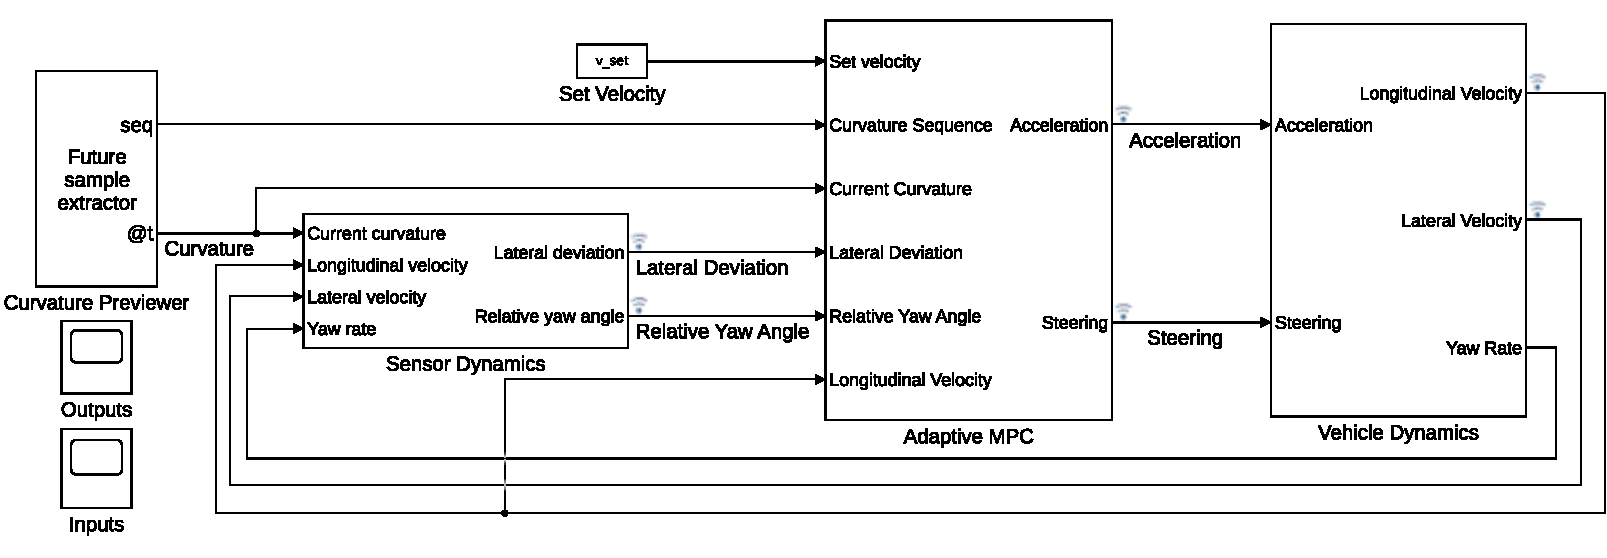
\includegraphics[width=\textwidth]{./figure/lane_following_AMPC.pdf}
	\caption{Overall procedure scheme lane following.}
	\label{fig:scheme_lane_following}
\end{figure}

This control scheme is composed by four different blocks that are the Sensor Dynamics, the Vehicle Dynamics, the Adaptive MPC controller and the Curvature Previewer.
Summarizing, the Vehicle Dynamics applies the bicycle model of lateral vehicle dynamics and approximate the longitudinal dynamics using a time constant according to what was seen previously; the Sensor Dynamics approximates a sensor, such as a camera or a laser, to calculate the lateral deviation and relative yaw angle; the Curvature Previewer detects the curvature at the current time step and the curvature sequence over the prediction horizon of the MPC controller and finally Adaptive MPC generates the optimal control inputs for a lane following system. The objective of the trajectory planning along specified path can be described as follows: given a path which the vehicle is expected to follow design a trajectory of a car-vehicle configuration.
In order to do this it is possible to derive the road curvature and its derivative.
For a plane curve given parametrically in Cartesian coordinates as $\gamma(t)=(x(t),y(t))$, the signed curvature is 
\begin{equation}
\label{eqn:curvature}
\kappa=\frac{x'y''-x''y'}{(x'^2+y'^2)^\frac{3}{2}}
\end{equation}
where primes refer to derivatives $\frac{d}{dt}$ with respect to the parameter $t$. The resulting curvature (\ref{eqn:curvature}) is a rational function, continuous except at the roots of the denominator, which is always nonzero provided that the interpolated positions do not contain subsequent duplicate values and that the points are spaced sufficiently \cite{longitudinal}.
The vehicle dynamics is represented by a Simulink model in Figure \ref{fig:scheme_lane_following_vehicle_dynamics}  where on the upper part we find the longitudinal dynamics while on the lower part we can see the lateral dynamics highlighted by the gains that are the components of the linear discrete state-space model (\ref{eqn:lateral_dynamics_simple_model}).
 
%VEHICLE DYNAMICS
\begin{figure}[!h]
	\centering
	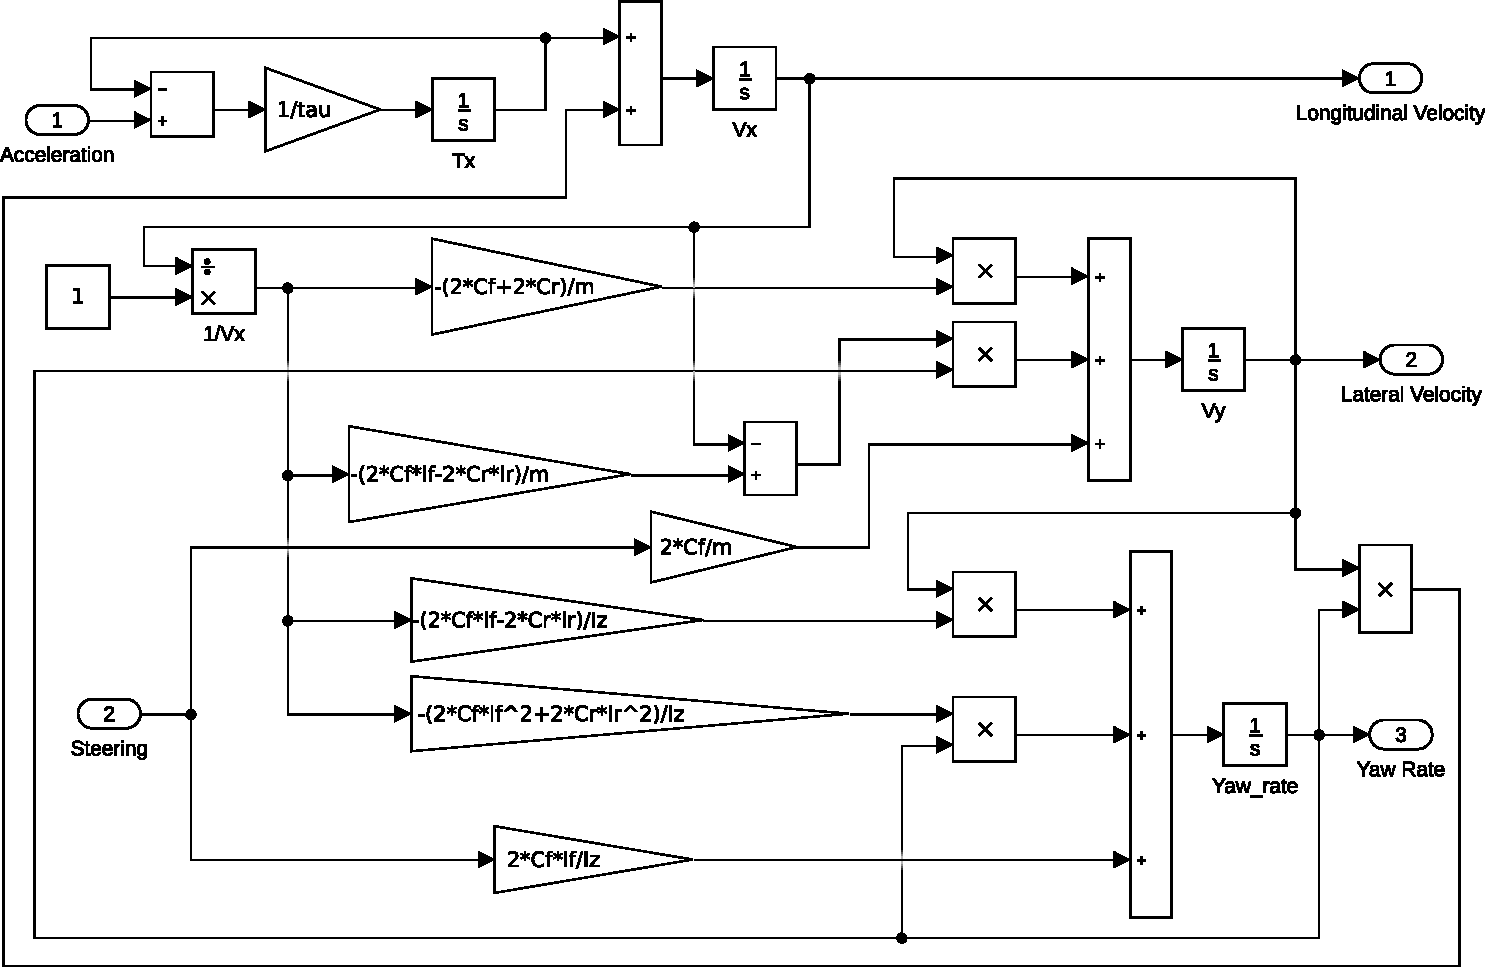
\includegraphics[width=\textwidth]{./figure/lane_following_AMPC_vehicle_dynamics.pdf}
	\caption{Vehicle Dynamics of the overall scheme lane following.}
	\label{fig:scheme_lane_following_vehicle_dynamics}
\end{figure}
We created an Adaptive MPC controller with a prediction model that has six states, three outputs (longitudinal velocity, lateral deviation, relative yaw angle), two manipulated signals (acceleration and steering) and one measured disturbance (desired yaw rate).

In order to design a valid lane keeping algorithm based on MPC we have set the constraints for manipulated variables and the scale factors. In particular the control
variables are constrained as follows:
\begin{equation}
\label{eqn:constraint_LKA}
\begin{array}{cc}
	\SI{-3}{m/s^2}\leq a\leq\SI{3}{m/s^2}\qquad\quad
	\SI{-1.13}{rad}\leq \delta \leq \SI{1.13}{rad}\;,
\end{array}
\end{equation}

Moreover we have specified the weights in the standard MPC cost function. The third output, yaw angle, is allowed to float because there are only two manipulated variables to make it a square system. In this controller, there is no steady-state error in the yaw angle as long as the second output, lateral deviation, reaches 0 at steady state. Finally we have also penalized acceleration change more for smooth driving experience. This controller uses a linear model for the vehicle dynamics and updates the model online as the longitudinal velocity varies.
The dynamics of the sensors (Figure \ref{fig:scheme_lane_following_sensor_dynamics}) allows us to calculate two fundamental parameters to reach the goal of keeping the vehicle in its lane and following the curved road by controlling the front steering angle:
\begin{itemize}
	\item $e_1$ which is the offset to the center line,
	\item $e_2$ which is the relative angle to the center line.
\end{itemize}
where we want to drive the yaw angle error and the lateral displacement error to zero to achieve our goal. The product of the road curvature and the longitudinal velocity is modeled as a measured disturbance.
%SENSOR DYNAMICS
\begin{figure}[!h]
	\centering
	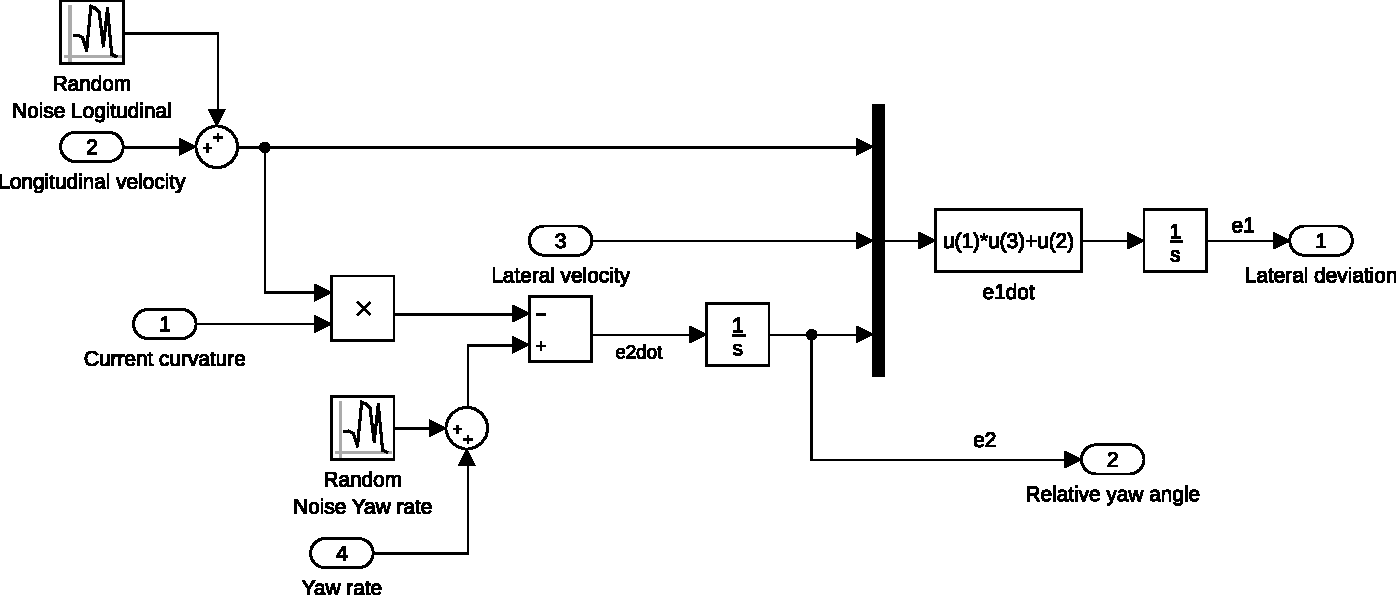
\includegraphics[width=\textwidth]{./figure/lane_following_AMPC_sensor_dynamics.pdf}
	\caption{Sensor Dynamics of the overall scheme lane following.}
	\label{fig:scheme_lane_following_sensor_dynamics}
\end{figure}

\section{Simulation Results}
The proposed adaptive MPC algorithm is designed in the MATLAB/Simulink and validated through simulations considering different paths. The objective of these tests is to evaluate the behavior of the proposed control strategy in critical situations. The parameters used in the lane following simulations are summarized in table \ref{tab:params}:
\begin{table}[!h]
	\centering
	\begin{tabular}{|c|c|c|}
		\hline
		\bfseries Parameters          & \bfseries Values   & \bfseries Description   \\
		\hline
		$m$          & \SI{1575}{kg}  & Mass of the vehicle            \\
		$I_z$         & \SI{2875}{kgm^2}   & Inertia Moment            \\
		$l_F$           & \SI{1.2}{m}     & Distance from COG to front axle         \\
		$l_R$         & \SI{1.6}{m}    & Distance from COG to rear axle           \\
		$C_F$          & \SI{19000}{\newton/rad}&Front cornering stiffness      \\
		$C_R$           & \SI{33000}{\newton/rad}&Rear cornering stiffness  \\
		$\tau$             & \SI{0.2}    & Time constant            \\
		$V_0$           & \SI{15}{m/s} & Initial Velocity      \\
		$V_{\text{set}}$          & \SI{20}{m/s} & Driver-set Velocity  \\
		$T_s$         & \SI{0.02}{s} & Sampling Time
		         \\
		\hline
	\end{tabular}
	\caption{Parameters of Vehicle Dynamics and Road Curvature.}
	\label{tab:params}
\end{table}

The paths considered for the evaluation of the proposed control strategy are:
\begin{itemize}
	\item a \textit{double lane change} curve (useful when a vehicle has to pass an obstacle), 
	\item a \textit{sinusoidal} path (slalom cones scenario),
	\item a \textit{circular/elliptic} path (NASCAR race tracks).
\end{itemize} 

\subsection{Double Lane Change Path}
In the first simulation the desired path is described in terms of the lateral position $Y_\text{ref}$ as function of the
longitudinal position $X_\text{ref}$. The equations (\ref{eqn:double_lane_change}) describe a double lane change that have
been employed in different tests for different scenarios i.e. \cite{Falcone2007a} \cite{Falcone2007b} \cite{Falcone2006} as follow :
\begin{equation}
\label{eqn:double_lane_change}
\begin{array}{cccc}
X_\text{ref}=V_x\cdot t, \quad\text{with}\quad t\in[0,10]\SI{}{s} \\\\
z_1 = \displaystyle
\frac{2.4}{50}(X_\text{ref}-27.19)-1.2;\quad
z_2=\displaystyle\frac{2.4}{43.9}(X_\text{ref}-56.46)-1.2;\\\\
Y_\text{ref}=\displaystyle\frac{8.1}{2}(1+\tanh(z_1)) - \frac{8.4}{2}(1+\tanh(z_2)).
\end{array}
\end{equation}
Figures \ref{fig:reference_laneFollowing_curve} and \ref{fig:curvature_laneFollowing_curve} represent the first trajectory that the vehicle must perform and the curvature calculated with the previous formula \ref{eqn:curvature}. 

%LANE FOLLOWING SIMPLE CURVE - PATH/CURVATURE
\begin{figure}[!h]
	\begin{minipage}[t]{0.5\textwidth}
		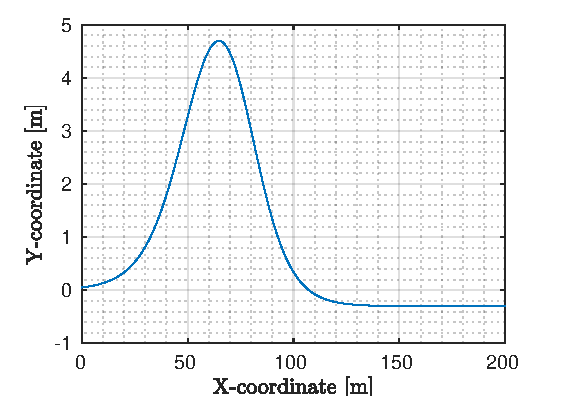
\includegraphics[width=\textwidth]{../../MATLAB/lane_following_curve/figure/Reference_curve.pdf}
		\subcaption{}
		\label{fig:reference_laneFollowing_curve}
	\end{minipage}
	\begin{minipage}[t]{0.5\textwidth}
		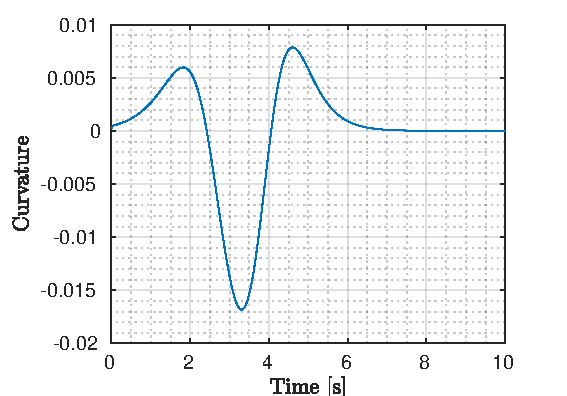
\includegraphics[width=\textwidth]{../../MATLAB/lane_following_curve/figure/Curvature_curve.pdf}
		\subcaption{}
		\label{fig:curvature_laneFollowing_curve}
	\end{minipage}
	\caption{Desired double lane change path and its curvature of the ATLASCAR2 in a simulation of \SI{10}{s} with initial position in $(0,0)$.}
	\label{fig:laneFollowing_desired_curve}
\end{figure}
From the following figures, on the other hand, it can be deduced that the control system we have created allows the ATLASCAR2 to respect the imposed constraints and to reach the set objectives. The longitudinal and lateral components of the velocity are represented in figures \ref{fig:longitudinal_velocity_laneFollowing_curve} and \ref{fig:lateral_velocity_laneFollowing_curve}. In the first few seconds of the simulation $V_x$ increases thanks to a constant acceleration imposed by the first input (Figure \ref{fig:acceleration_laneFollowing_curve}). Later this acceleration decreases converging to zero so that at run time, we can note that $V_x$ reaches the predefined value of \SI{20}{m/s} and then it stabilizes near the driver set velocity because it continues to vary the steering angle to adapt to the path to be followed (Figure \ref{fig:steering_laneFollowing_curve}). The lateral component $V_y$, on the other hand, only affects during the steering phase when we are forcing a change of direction.
%LANE FOLLOWING SIMPLE CURVE - PATH/CURVATURE
\begin{figure}[!h]
	\begin{minipage}[t]{0.5\textwidth}
		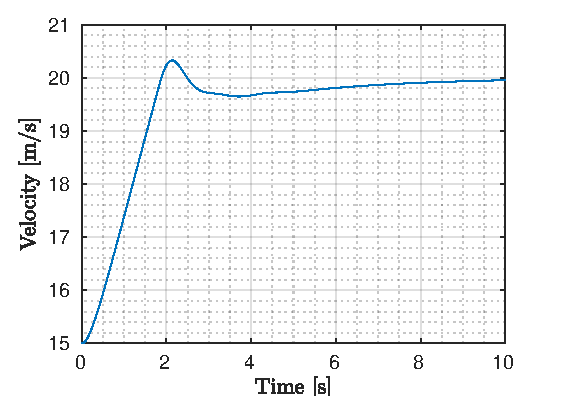
\includegraphics[width=\textwidth]{../../MATLAB/lane_following_curve/figure/LongitudinalVelocityVsTime_curve.pdf}
		\subcaption{Longitudinal velocity $V_x$ w.r.t. time.}
		\label{fig:longitudinal_velocity_laneFollowing_curve}
	\end{minipage}
	\begin{minipage}[t]{0.5\textwidth}
		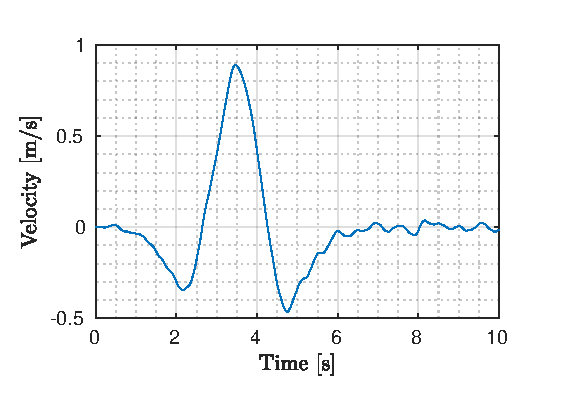
\includegraphics[width=\textwidth]{../../MATLAB/lane_following_curve/figure/LateralVelocityVsTime_curve.pdf}
		\subcaption{Lateral velocity $V_y$ w.r.t. time.}
		\label{fig:lateral_velocity_laneFollowing_curve}
	\end{minipage}
	\begin{minipage}[t]{0.5\textwidth}
		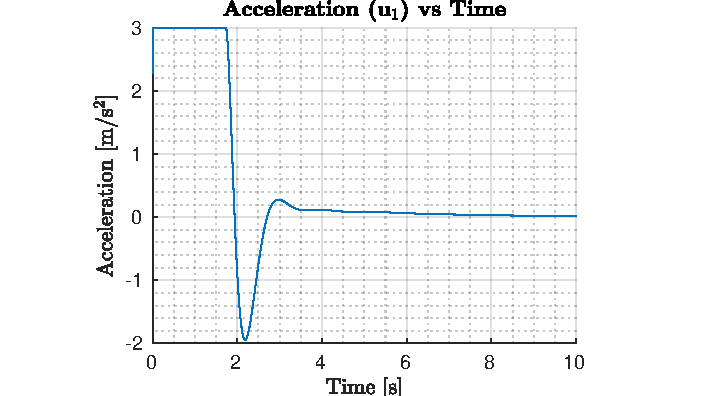
\includegraphics[width=\textwidth]{../../MATLAB/lane_following_curve/figure/AccelerationVsTime_curve.pdf}
		\subcaption{Acceleration $u_1$ w.r.t. time.}
		\label{fig:acceleration_laneFollowing_curve}
	\end{minipage}
	\begin{minipage}[t]{0.5\textwidth}
		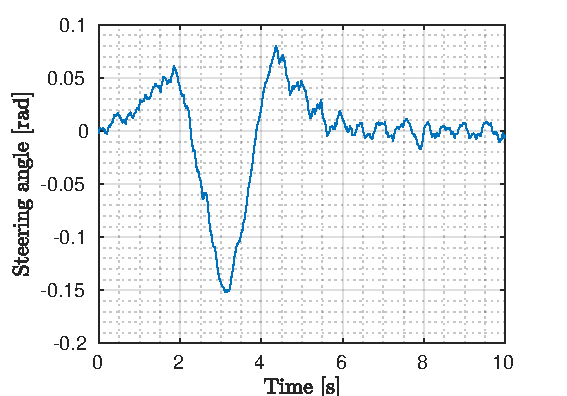
\includegraphics[width=\textwidth]{../../MATLAB/lane_following_curve/figure/SteeringAngleVsTime_curve.pdf}
		\subcaption{Steering angle $u_2$ w.r.t. time.}
		\label{fig:steering_laneFollowing_curve}
	\end{minipage}
	\begin{minipage}[t]{0.5\textwidth}
		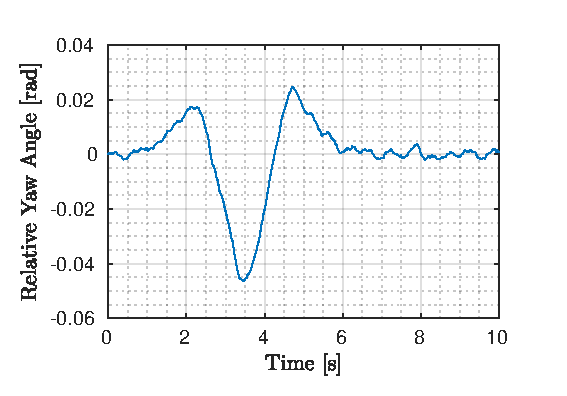
\includegraphics[width=\textwidth]{../../MATLAB/lane_following_curve/figure/RelativeYawAngleVsTime_curve.pdf}
		\subcaption{Relative yaw angle $e_2$ w.r.t. time.}
		\label{fig:relative_yaw_angle_laneFollowing_curve}
	\end{minipage}
	\begin{minipage}[t]{0.5\textwidth}
		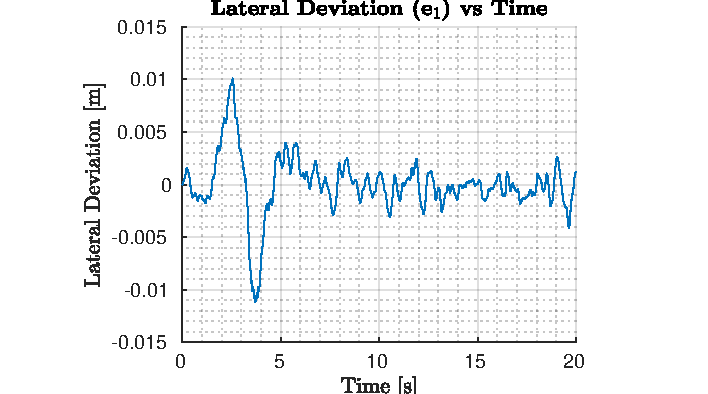
\includegraphics[width=\textwidth]{../../MATLAB/lane_following_curve/figure/LateralDeviationVsTime_curve.pdf}
		\subcaption{Lateral deviation $e_1$ w.r.t. time.}
		\label{fig:lateral_deviation_laneFollowing_curve}
	\end{minipage}
	\caption{Time signals of the ATLASCAR2 in the simulation with a double lane change
		 path.}
	\label{fig:laneFollowing_signals_curve}
\end{figure}
From Figures \ref{fig:lateral_deviation_laneFollowing_curve} and \ref{fig:relative_yaw_angle_laneFollowing_curve} we can notice that the lateral deviation and the relative yaw angle both converge to zero. That is, the ATLASCAR2 follows the road closely based on the previewed curvature.
\newpage
\subsection{Sinusoidal Path}
In the second simulation we assumed that the car must follow a sinusoidal path. We have extended the simulation time to 20 seconds in order to better understand the progress of the various signals. Figures \ref{fig:reference_laneFollowing} and \ref{fig:curvature_laneFollowing} show the desired path and its curvature, where the former is described in terms of the lateral position $Y_{\text{ref}}$ as function of the longitudinal position $X_{\text{ref}}$ and the latter is derived according with \cite{curvature}. The ATLASCAR2 is controlled to follow a sinusoidal trajectory which is given as follows:
\begin{equation}
\begin{aligned}
X_\text{ref}&=V_x\cdot t,\quad \text{with}\quad t\in[0,20]\SI{}{s}\\
Y_\text{ref}&=\displaystyle 5\sin\Big(\frac{X_\text{ref}}{20}\Big) 
\end{aligned}
\end{equation}
%LANE FOLLOWING SINUSOIDAL PATH - PATH/CURVATURE
\begin{figure}[!h]
	\begin{minipage}[t]{0.5\textwidth}
		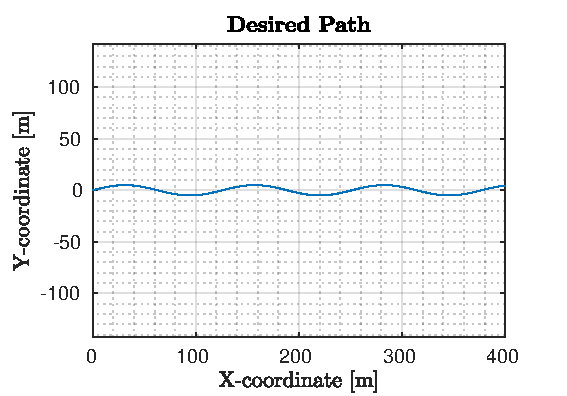
\includegraphics[width=\textwidth]{../../MATLAB/lane_following/figure/Reference.pdf}
		\subcaption{}
		\label{fig:reference_laneFollowing}
	\end{minipage}
	\begin{minipage}[t]{0.5\textwidth}
		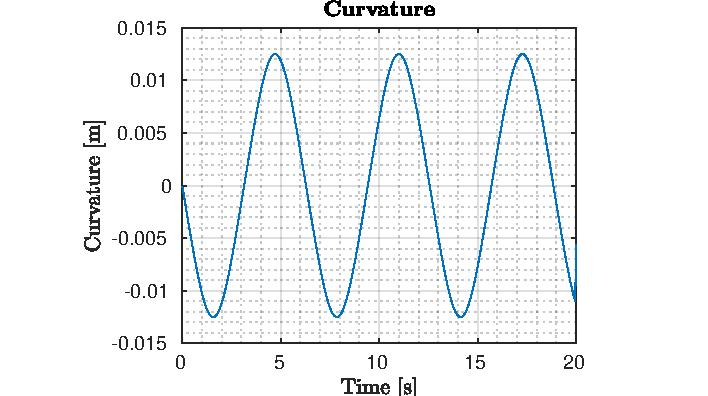
\includegraphics[width=\textwidth]{../../MATLAB/lane_following/figure/Curvature.pdf}
		\subcaption{}
		\label{fig:curvature_laneFollowing}
	\end{minipage}
	\caption{Desired sinusoidal path and its curvature of the ATLASCAR2 in a simulation of \SI{20}{s}.}
	\label{fig:laneFollowing_desired}
\end{figure}

In practice this type of route can be followed by the vehicle when it has to make a slalom between cones or it must go up some hairpin bends in the mountains. Moreover the following figures show the trend of the main parameters confirming that the control strategy used allows the vehicle to follow the path. In particular we simulated also a small error in the sensor dynamics in order to make the simulation more realistic: we added a 3 percent error to the longitudinal velocity and this is evident from the small noise in the graphs of the steering angle (Figure \ref{fig:steering_laneFollowing}) and the lateral deviation (Figure \ref{fig:lateral_deviation_laneFollowing}).
Figure {\ref{fig:longitudinal_velocity_laneFollowing}} shows the evolution of the vehicle longitudinal velocity. Also in this simulation the velocity is equal to the initial condition for longitudinal velocity parameter $V_0$. At run time, we can note that $V_x$ reaches the predefined value of \SI{20}{m/s} and then it stabilizes near the cruising speed because it continues to vary the steering angle to adapt to the path to be followed. In this scenario the lateral deviation and the relative angle yaw do not converge to zero but oscillate. We can however assert that this type of oscillation is due to the type of path we are following. Furthermore the limits of this oscillation are very small indeed: in particular the lateral deviation is less than \SI{1.5}{cm} while the maximum relative yaw angle is \SI{0.04}{rad}. We can therefore state that even in this case the vehicle correctly follows the lane.
%LANE FOLLOWING SINUSOIDAL PATH - SIGNALS
\begin{figure}[!h]
	\begin{minipage}[t]{0.5\textwidth}
		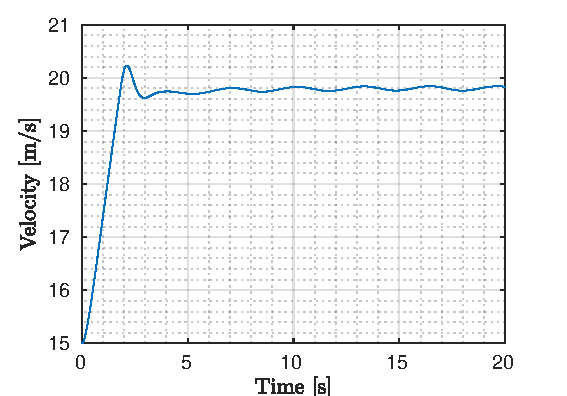
\includegraphics[width=\textwidth]{../../MATLAB/lane_following/figure/LongitudinalVelocityVsTime.pdf}
		\subcaption{Longitudinal velocity $V_x$ w.r.t. time.}
		\label{fig:longitudinal_velocity_laneFollowing}
	\end{minipage}
	\begin{minipage}[t]{0.5\textwidth}
			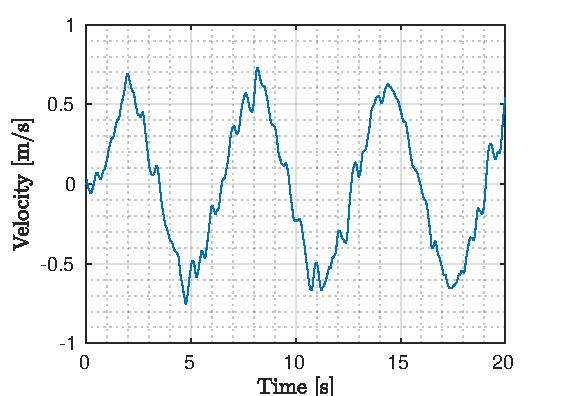
\includegraphics[width=\textwidth]{../../MATLAB/lane_following/figure/LateralVelocityVsTime.pdf}
			\subcaption{Lateral velocity $V_y$ w.r.t. time.}
			\label{fig:lateral_velocity_laneFollowing}
	\end{minipage}
	\begin{minipage}[t]{0.49\textwidth}
		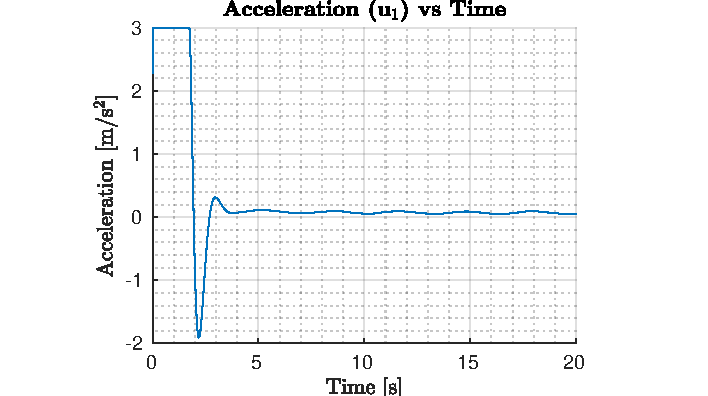
\includegraphics[width=\textwidth]{../../MATLAB/lane_following/figure/AccelerationVsTime.pdf}
		\subcaption{Acceleration $u_1$ w.r.t. time.}
		\label{fig:acceleration_laneFollowing}
	\end{minipage}
	\begin{minipage}[t]{0.49\textwidth}
		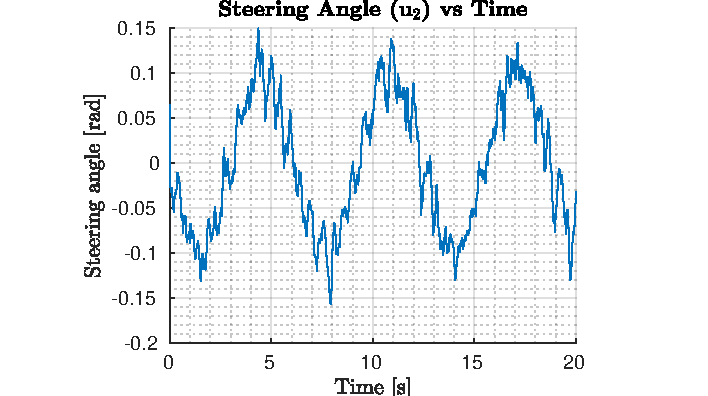
\includegraphics[width=\textwidth]{../../MATLAB/lane_following/figure/SteeringAngleVsTime.pdf}
		\subcaption{Steering angle $u_2$ w.r.t. time.}
		\label{fig:steering_laneFollowing}
	\end{minipage}
	\begin{minipage}[t]{0.49\textwidth}
		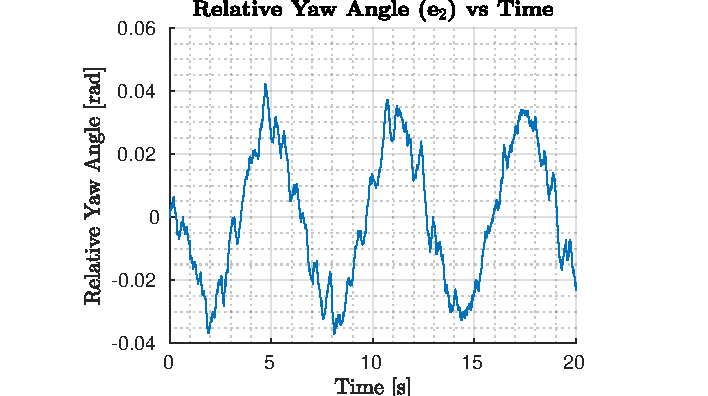
\includegraphics[width=\textwidth]{../../MATLAB/lane_following/figure/RelativeYawAngleVsTime.pdf}
		\subcaption{Relative yaw angle $e_2$ w.r.t. time.}
		\label{fig:relative_yaw_angle_laneFollowing}
	\end{minipage}
	\begin{minipage}[t]{0.49\textwidth}
		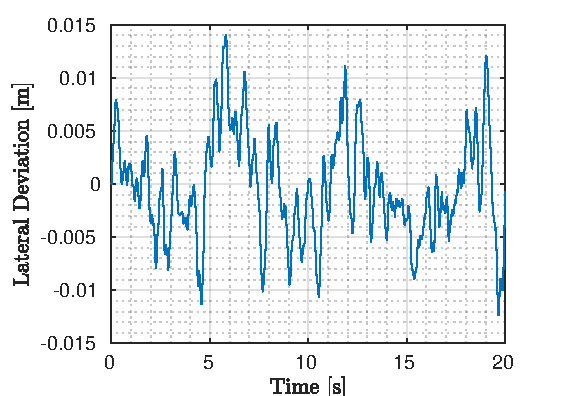
\includegraphics[width=\textwidth]{../../MATLAB/lane_following/figure/LateralDeviationVsTime.pdf}
		\subcaption{Lateral deviation $e_1$ w.r.t. time.}
		\label{fig:lateral_deviation_laneFollowing}
	\end{minipage}
	\caption{Time signals of the ATLASCAR2 in the simulation with a sinusoidal path.}
	\label{fig:laneFollowing_signals}
\end{figure}

\subsection{Circular/Elliptic Path}
In the last simulation we considered that the vehicle must follow an elliptic path with a semi-major axis of \SI{30}{m} and semi-minor axis of \SI{15}{m} depicted in Figure \ref{fig:reference_laneFollowing_circular}. Also in this case the simulation time is \SI{20}{s}.
To describe the elliptic path and to evaluate its curvature, depicted in Figure \ref{fig:curvature_laneFollowing_circular}, the equations are as follows:
\begin{equation}
	X_\text{ref}=\displaystyle 15\cos\Bigg(\frac{V_x\cdot t}{60}\Bigg) \qquad
	Y_\text{ref}=\displaystyle 30\sin\Bigg(\frac{V_x\cdot t}{60}\Bigg)  
 \quad\text{with}\quad t\in[0,20]\SI{}{s}
\end{equation}
% ELLIPTIC PATH
\begin{figure}[!h]
	\begin{minipage}[t]{0.5\textwidth}
		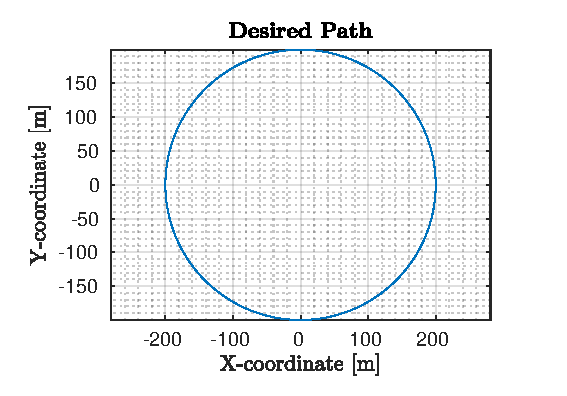
\includegraphics[width=\textwidth]{../../MATLAB/lane_following_circular_path/figure/Reference_circular.pdf}
		\subcaption{}
		\label{fig:reference_laneFollowing_circular}
	\end{minipage}
	\begin{minipage}[t]{0.5\textwidth}
		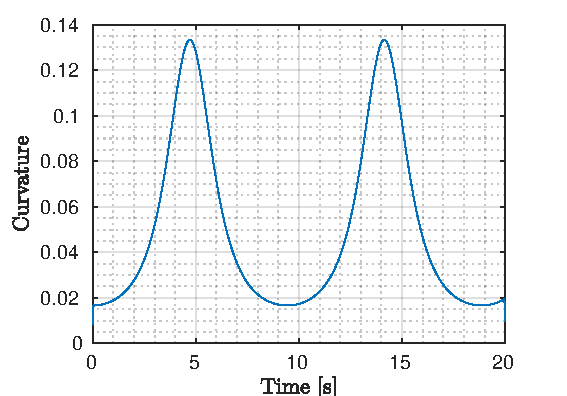
\includegraphics[width=\textwidth]{../../MATLAB/lane_following_circular_path/figure/Curvature_circular.pdf}
		\subcaption{}
		\label{fig:curvature_laneFollowing_circular}
	\end{minipage}
	\caption{Desired elliptic path and its curvature of the ATLASCAR2 in a simulation of \SI{20}{s} with initial position in $(0,30)$.}
	\label{fig:laneFollowing_desired_circular}
\end{figure}

In particular in Figure \ref{fig:laneFollowing_signals_circular} are represented the time signals of the ATLASCAR2 in the simulation with the elliptic path. It is possible to notice that also in this case the vehicle follows the path with a minimal lateral deviation described in the Figure \ref{fig:lateral_deviation_laneFollowing_circular}.

However, the minimum lateral displacement is at the expense of the costant cruise velocity; infact Figure \ref{fig:longitudinal_velocity_laneFollowing_circular} and \ref{fig:lateral_velocity_laneFollowing_circular} show an oscillatory pattern of both longitudinal speed and lateral velocity caused by the continuous change of direction of the road and the length of the latter. 

Also in this situation we simulated a small error in the sensor dynamics in order to make the scenario more realistic: we added a 2 percent error to the longitudinal velocity and this is evident from the small noise in the graphs of the steering angle (Figure \ref{fig:steering_laneFollowing_circular}) and the lateral deviation (Figure \ref{fig:lateral_deviation_laneFollowing_circular}).

As previously stated, the vehicle follows the lane and allows us to state that the control system we have designed is efficient and robust.
%LANE FOLLOWING ELLIPTIC - PATH/CURVATURE
\begin{figure}[!h]
	\begin{minipage}[t]{0.5\textwidth}
		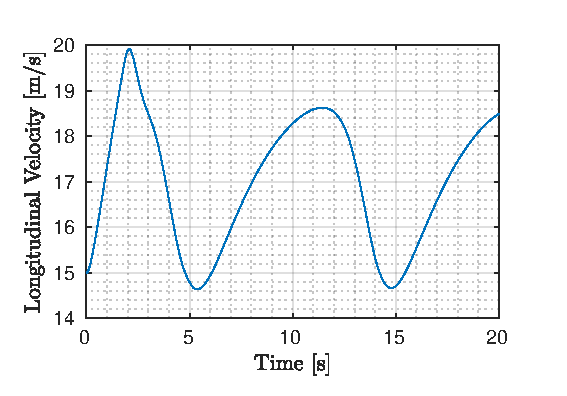
\includegraphics[width=\textwidth]{../../MATLAB/lane_following_circular_path/figure/LongitudinalVelocityVsTime_circular.pdf}
		\subcaption{Longitudinal velocity $V_x$ w.r.t. time.}
		\label{fig:longitudinal_velocity_laneFollowing_circular}
	\end{minipage}
	\begin{minipage}[t]{0.5\textwidth}
		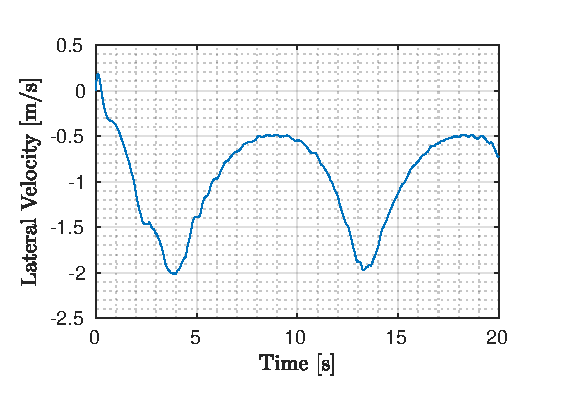
\includegraphics[width=\textwidth]{../../MATLAB/lane_following_circular_path/figure/LateralVelocityVsTime_circular.pdf}
		\subcaption{Lateral velocity $V_y$ w.r.t. time.}
		\label{fig:lateral_velocity_laneFollowing_circular}
	\end{minipage}
	\begin{minipage}[t]{0.5\textwidth}
		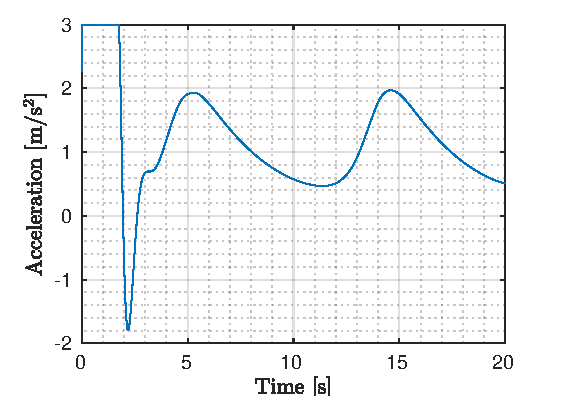
\includegraphics[width=\textwidth]{../../MATLAB/lane_following_circular_path/figure/AccelerationVsTime_circular.pdf}
		\subcaption{Acceleration $u_1$ w.r.t. time.}
		\label{fig:acceleration_laneFollowing_circular}
	\end{minipage}
	\begin{minipage}[t]{0.5\textwidth}
		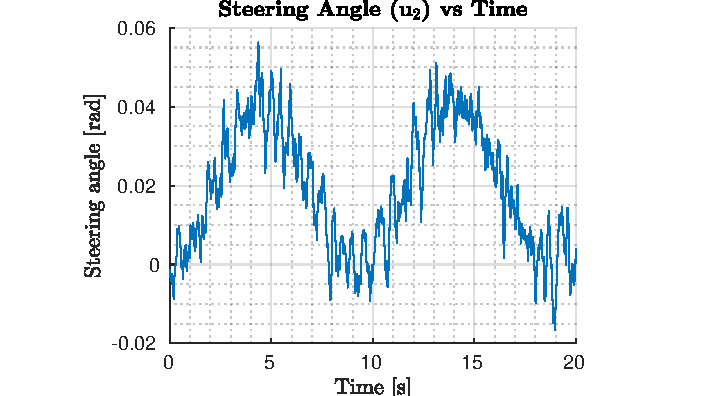
\includegraphics[width=\textwidth]{../../MATLAB/lane_following_circular_path/figure/SteeringAngleVsTime_circular.pdf}
		\subcaption{Steering angle $u_2$ w.r.t. time.}
		\label{fig:steering_laneFollowing_circular}
	\end{minipage}
	\begin{minipage}[t]{0.5\textwidth}
		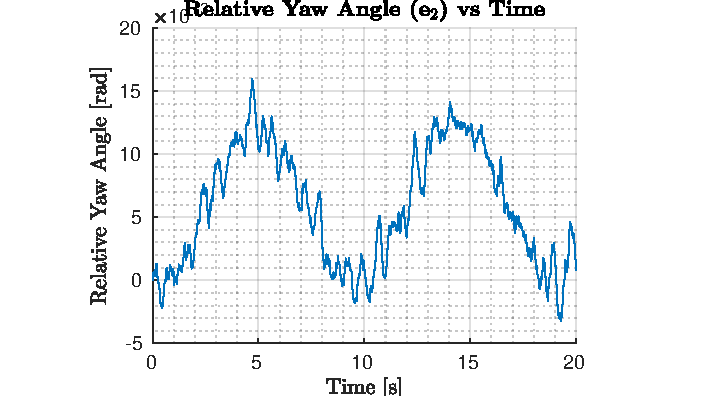
\includegraphics[width=\textwidth]{../../MATLAB/lane_following_circular_path/figure/RelativeYawAngleVsTime_circular.pdf}
		\subcaption{Relative yaw angle $e_2$ w.r.t. time.}
		\label{fig:relative_yaw_angle_laneFollowing_circular}
	\end{minipage}
	\begin{minipage}[t]{0.5\textwidth}
		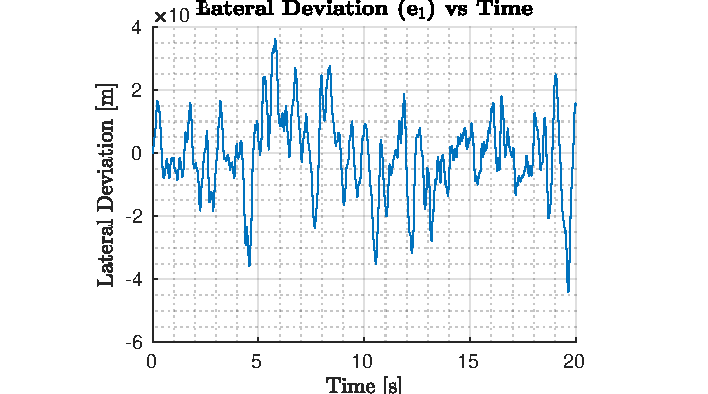
\includegraphics[width=\textwidth]{../../MATLAB/lane_following_circular_path/figure/LateralDeviationVsTime_circular.pdf}
		\subcaption{Lateral deviation $e_1$ w.r.t. time.}
		\label{fig:lateral_deviation_laneFollowing_circular}
	\end{minipage}
	\caption{Time signals of the ATLASCAR2 in the simulation with an elliptic path.}
	\label{fig:laneFollowing_signals_circular}
\end{figure}


%%%CIAOOOOOOOOOOOOOOOOOOOOOOOOOOOOOOOOOOOOOOOOOO

